\documentclass[12pt,a4paper]{article}
\usepackage{lipsum}
\usepackage{authblk}
\usepackage[top=2cm, bottom=2cm, left=2cm, right=2cm]{geometry}
\usepackage{tocloft}
\usepackage{color}
\usepackage{hyperref}
\usepackage{filecontents}
\usepackage{listings}
\usepackage{tikz}
\usetikzlibrary{calc,shapes.multipart,chains,arrows}

% end of package imports

\renewenvironment{abstract}{%
\hfill\begin{minipage}{0.95\textwidth}
\rule{\textwidth}{1pt}}
{\par\noindent\rule{\textwidth}{1pt}\end{minipage}}
%
\makeatletter
\renewcommand\@maketitle{%
    \hfill
    \begin{minipage}{0.95\textwidth}
    \vskip 2em
    \let\footnote\thanks 
    {\LARGE \@title \par }
    \vskip 1.5em
    {\large \@author \par}
    \end{minipage}
    \vskip 1em \par
}
\makeatother

\renewcommand*\contentsname{Table of contents}

%-------definitions-----
\newcommand{\Author}{Kyle Kersey}
\newcommand{\Title}{Note Chain Project}
\newcommand{\Keywords}{}
%--------------------------

%title and author details
\title{\textbf{\Title}}
\author{\Author}
\date{}


\pdfinfo{
   /Author (\Author)
   /Title  (\Title)
   /Keywords (\Keywords)
   /Date (May 2016)
}

\hypersetup{
	colorlinks,
	linktoc=all,
	linkcolor=black
}

\lstset{
	columns=flexible,
	basicstyle=\ttfamily
}

\definecolor{light-gray}{gray}{0.95}
\newcommand{\codetext}[1]{\colorbox{light-gray}{\texttt{#1}}}

\tikzset{
    squarecross/.style={
        draw, rectangle,minimum size=18pt,
        inner sep=0pt, text=black,
        path picture = {
            \draw[black]
            (path picture bounding box.north west) --
            (path picture bounding box.south east)
            (path picture bounding box.south west) --
            (path picture bounding box.north east);
        }
    },
     connect/.style={-latex, thick},
     list/.style={
            very thick, rectangle split,
            rectangle split parts=4, draw,
            rectangle split horizontal, minimum size=18pt,
            inner sep=4pt, text=black
        },
        ->, start chain, very thick
}


\begin{document}


\clearpage
\maketitle
%
\begin{abstract}
A note taking tool for managing simple text based notes containing many version
control features for managing revisions such as branching, commits. The
software is written in the Ada programming language and has a modular design
allowing use of different storage systems.
\end{abstract}

\renewcommand\cftsecleader{\cftdotfill{\cftdotsep}}

\tableofcontents
\thispagestyle{empty}
\pagebreak
\setcounter{page}{1}


\section{Project structure}

\subsection{Introduction}
The main source files are in the \codetext{src} directory and the compiled
result is put in the \codetext{obj} directory along with the object files and
other intermediate compiled files. Unit tests are in the \codetext{tests}
directory.

\subsection{Source files}
\subsubsection{main.adb}
This is the main file which loads the other packages and decides how to
interact with the other packages based on the command line arguments supplied
by the user. At the bottom of the file is a series of if else statements to
call a procedure for responding to a command. the methods which interact with a
command will by convention start with the \codetext{Cmd\_} prefix. When it
first starts it will call the \codetext{Init} procedure in the client package
passing in the database object as a parameter. At the end of the declaration
section a variable named \codetext{Data\_DB} which is the implementation of
Key-Value database being used. When Done the database connection is cleaned up.

\subsubsection{client.ads}
This package implements the main operations used in the project and is called
by \codetext{main.adb} at the start of the file the data types used in the
project are declared then the functions and procedures to operate on those
types. To make the system more modular this package is independent of the
database system being used and and will work with any Key-Value database which
implements the interface \codetext{KV\_Container}. Each of the methods which
interact with data need to be passed the variable containing the database, the
access mode to this variable needs to be \codetext{in out} write even for
operations which only read data because the database object might need to be
modified such as caching frequently used data.

\subsubsection{config.ads}
This package contains constant variables for project configuration values such
as the version number and paths of where the project data is stored, file paths
are made cross platform for Windows or Unix.

\subsubsection{file\_operations.ads}
Reusable operations for files are declared in this package such as writing to a
file or getting the SHA-256 hash of a file this package also contains an
operation called \codetext{Execute\_System\_Cmd} runs a shell command.

\subsubsection{settings.ads}
This stores the settings created by the user, the values are stored as key-value
pairs in a hash map data structure then serialized to JSON when storing or
loading from a file. The config package contains a constant named
\codetext{Settings\_JSON\_File} which defines where this file is located. When a
setting key is requested which does not exist then a \codetext{No\_Key\_Error}
is raised.

\subsubsection{object\_store.ads}
Data is stored as as objects, this package contains operations on these objects
such as loading and reading them from the Key-Value database, objects are
identified by their SHA-256 hash. the methods in this package accept the
database as Key-Value database as the first parameter. when an object cannot be
found then a \codetext{Object\_Not\_Found} exception is raised. The exact format
of an object is described in a later section.

\subsubsection{string\_operations.ads}
Reusable operations on strings are declared in this package such as converting a
time object to and from a text format, it also has functions for searching in a
string and validating the format of a SHA-256 hash.

\subsubsection{note\_interactive\_menu.ads}
this shows a visual interactive menu to select a note. it returns the SHA-256
hash of the selected note, it uses the VIM editor to implement this.

\subsubsection{data\_store/kv\_store.ads}
This package defines an interface for
Key-Value databases, new Key-Value databases must implement this interface to be
used with the system. The interface ensures that child packages will implement
operations such as set, get, remove and check if items exist the data store. It
also has a procedure to commit values if the database being used as transactions
which need to be committed to permanent storage. The procedure \codetext{Setup}
is called to load the database and \codetext{Cleanup} is called when the
database is done being used. If a requested item cannot be found in the database
then the exception \codetext{No\_Key\_Error} should be raised. The name of a
Key-Value store implementation is returned by the function \codetext{Name}.

\subsection{Unit tests}
Unit tests are done with the Aunit testing framework
\cite{Aunit},  a test is written for each major package to unsure that the
methods operate properly. For testing the data is stored in memory using a hash
map key-value store.

\subsection{Data types and structures}
The main three data types used for the
data are: Commit, Note and Tree. Each of These are record types which inherit
from the Object\_Record type. Interface types are used to ensure that each of
these data records will implement operations for working with the database. Ada
does not have multiple inheritance, but does it allow for implementing multiple
interfaces  \cite{Ada-Interface-Types}. The Interface \codetext{Persistable} is
inherits from the types \codetext{JSON\_Serializable} and
\codetext{Storable\_Object} this ensures that each of the record types which
inherit from this interface will implement operations to serialize the data to
and from a JSON \cite{rfc7159} String. The Storable\_Object interface makes
records implement a procedure for saving to the database and a function for
fetching an item from the database by it's SHA-256 hash. 

\par All data is stored in an immutable data structure called a Merkle tree,
each leaf in the tree contains the hash of the children leafs. A list of tree
head nodes is maintained in a JSON file each item references a different branch
name. The head node points to a commit object. A commit object contains when it
was created, it's entry tree object reference and the next commit references. The
commits are like a liked list in that each item points to the next, 
but a commit can have multiple parents such as in the case of a merge. The tree
object contains a list of entries in that tree. Each entry has the type and
reference of the entry, such as a Note object or another child tree. All data
records items are stored as a JSON object. Before an item is put into the
database it is prefixed with the object type name in lower case then the length
of the data and a unix new line character then the Data Objects's content
begins. This format is taken from how the git version control system stores
items.

\subsubsection{Branches}
This is an example of the JSON file that stores information about the branches,
the \codetext{head} key stores the name of the current branch which in this
example is \textit{test}, the \codetext{branches} key contains a JSON object
where each key is a branch name.

\begin{verbatim}
{
  "branches": {
    "master": {
      "name": "master",
      "commit_ref": "(SHA-256 Hash)"
    },
    "test": {
      "name": "test",
      "commit_ref": "(SHA-256 Hash)"
    }
  },
  "head": "test"
}
\end{verbatim}



\section{Usage tutorial}
\subsection{Requirements}
An Ada compiler is required to build the project, it can be downloaded at
\href{http://libre.adacore.com/}{libre.adacore.com} or one can be installed on
Linux with the command \codetext{sudo apt-get install gnat}, the compiler also
needs Ada 2012 support. The vim text editor is required, it is used for editing
nodes and interactive menus. To build the unit tests the Aunit library needs to be installed.

\subsection{Building}
To build the executable run the following command in the project directory:

\begin{lstlisting}[language=bash]
  gprbuild -P note_chain.gpr
\end{lstlisting}

\noindent
this will output the executable to \codetext{./obj/note\_chain}, an exe file
extension will be added for Windows.

\par \noindent
To build the unit tests run the following command, this will output an
executable \codetext{./obj/tests/tests}.

\begin{lstlisting}[language=bash]
  gprbuild -P test.gpr
\end{lstlisting}

\subsection{Creating a new note}
To create a note run the command:

\begin{lstlisting}[language=bash]
  ./obj/note_chain note new
\end{lstlisting}

\noindent
This will open the vim editor, type out the content of the note, when done save
the contents and exit vim, this will create a new note. If you have trouble
with vim their are many tutorials online detailing the basic operations such as
how to save and exit.

\subsection{Listing notes}
To display all of the notes sorted by most recent run the command:

\begin{lstlisting}[language=bash]
  ./obj/note_chain note new
\end{lstlisting}


\subsection{Viewing notes}
To view a note using the interactive menu use the command:

\begin{lstlisting}[language=bash]
  ./obj/note_chain note menu
\end{lstlisting}

\noindent
This will open a temporary file in the vim editor, each line will contain the
SHA-256 of the note along with the date of when the note was created, the
selected line will be highlighted in red, use the arrow keys to navigate up and
down. Open the selected note with the return key. This will open the selected
note in the vim editor, any changes you make to this node will not be saved.

\subsection{Creating and changing branches}
To create a new branch from current use the following command:

\begin{lstlisting}[language=bash]
  ./obj/note_chain branch new <name>
\end{lstlisting}

\noindent
To change the branch use the command:

\begin{lstlisting}[language=bash]
  ./obj/note_chain branch checkout <name>
\end{lstlisting}


\subsection{Merging branches}
The commits of another branch can be merged into the current branch with the command:

\begin{lstlisting}[language=bash]
  ./obj/note_chain branch merge <name>
\end{lstlisting}

\subsection{Branch status}
To get the name of the current branch use the command:

\begin{lstlisting}[language=bash]
  ./obj/note_chain branch head
\end{lstlisting}

\noindent
To get a list of branch names use the command:

\begin{lstlisting}[language=bash]
  ./obj/note_chain branch list
\end{lstlisting}


\subsection{Settings}
Some settings can be defined such as the author name of the notes, values are
stored as a key-value pairs of strings in a JSON file. Settings are referenced
by their key name.

\subsubsection{Defining values}

\begin{lstlisting}[language=bash]
  ./obj/note_chain config set <key> <value>
\end{lstlisting}

\subsubsection{Getting values}

\begin{lstlisting}[language=bash]
  ./obj/note_chain config get <key>
\end{lstlisting}

\subsubsection{Listing}
This command will show all of the defined settings aligned into columns:

\begin{lstlisting}[language=bash]
  ./obj/note_chain config list
\end{lstlisting}

\subsubsection{Removing}
To remove a setting use the command:
\begin{lstlisting}[language=bash]
  ./obj/note_chain config remove <key>
\end{lstlisting}

\section{Future plans}
\subsection{Tree structure}

\begin{figure}[!h]
\centering

\begin{tabular}{|l|l}
 \cline{1-1}
	\hspace{1em} & item reference \\ \cline{1-1}
	& item type  \\ \cline{1-1}
	& modified node reference \\ \cline{1-1}
	& next node reference \\ \cline{1-1}
\end{tabular}


\caption{Entry structure}
\label{fig:M4}
\end{figure}


\begin{figure}[!h]
\centering
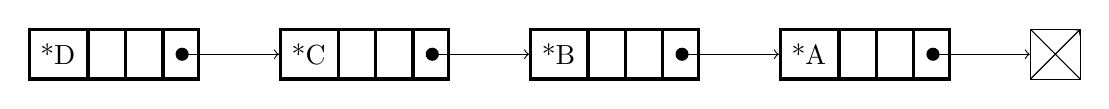
\begin{tikzpicture}

	\node[list,on chain] (A) {\nodepart{one}{*D}};
	\node[list,on chain] (B) {\nodepart{one}{*C}};
	\node[list,on chain] (C) {\nodepart{one}{*B}};
	\node[list,on chain] (D) {\nodepart{one}{*A}};

	  
	\node[squarecross]   (root) [right=of D] {};
	\draw[*->] let \p1 = (A.four), \p2 = (A.center) in (\x1,\y2) -- (B);
	\draw[*->] let \p1 = (B.four), \p2 = (B.center) in (\x1,\y2) -- (C);
	\draw[*->] let \p1 = (C.four), \p2 = (C.center) in (\x1,\y2) -- (D);
	\draw[*->] let \p1 = (D.four), \p2 = (D.center) in (\x1,\y2) -- (root);
\end{tikzpicture}
\caption{Entries created sequentially}
\label{fig:M1}
\end{figure}


\begin{figure}[!h]
\centering
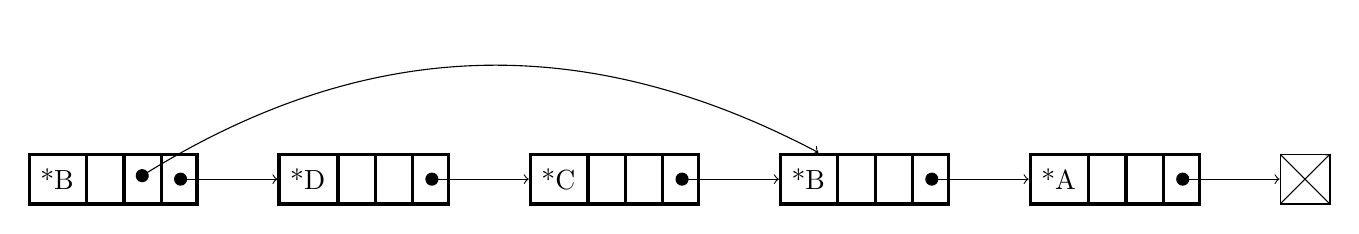
\begin{tikzpicture}

	\node[list,on chain] (A) {\nodepart{one}{*B}};
	\node[list,on chain] (B) {\nodepart{one}{*D}};
	\node[list,on chain] (C) {\nodepart{one}{*C}};
	\node[list,on chain] (D) {\nodepart{one}{*B}};
	\node[list,on chain] (E) {\nodepart{one}{*A}};
	  
	\node[squarecross]   (root) [right=of E] {};
	\draw[*->] let \p1 = (A.four), \p2 = (A.center) in (\x1,\y2) -- (B);
	\draw[*->] let \p1 = (B.four), \p2 = (B.center) in (\x1,\y2) -- (C);
	\draw[*->] let \p1 = (C.four), \p2 = (C.center) in (\x1,\y2) -- (D);
	\draw[*->] let \p1 = (D.four), \p2 = (D.center) in (\x1,\y2) -- (E);
	\draw[*->] let \p1 = (E.four), \p2 = (E.center) in (\x1,\y2) -- (root);	
	
	\path[*->] let \p1 = (A.three), \p2 = (A.center) in (\x1,\y2) edge [ bend left] (D);
\end{tikzpicture}
\caption{Updating an entry}
\label{fig:M2}
\end{figure}

\pagebreak

\begin{filecontents}{\jobname.bib}
@misc{Aunit,
  author = "AdaCore",
  title = {\textit{Ada unit testing framework}},
  url = "http://libre.adacore.com/tools/aunit/",
  year = "2016"
}

@techreport{Ada-Interface-Types,
	title = {\textit{The Implementation of Ada 2005 Interface Types in the GNAT Compiler}},
	author = "Javier Miranda and Edmond Schonberg and Gary Dismukes",
	year = 2005,
	institution = "AdaCore",
	url = "http://www.adacore.com/uploads/technical-papers/Ada-2005_Interface_Types.pdf"
}

@techreport{rfc7159,
	title = {\textit{The JavaScript Object Notation (JSON) Data Interchange Format}},
	author = "Douglas Crockford",
	HOWPUBLISHED = {Internet Requests for Comments},
	year = 2014,
	month = "March",
	PUBLISHER = "{RFC Editor}",
	TYPE = "{RFC}",
	NUMBER = 7159,
	INSTITUTION = "{RFC Editor}"
}
\end{filecontents}

\bibliographystyle{unsrt}
\bibliography{\jobname}

\end{document}
